\documentclass{standalone}
\usepackage{tikz}

\begin{document}

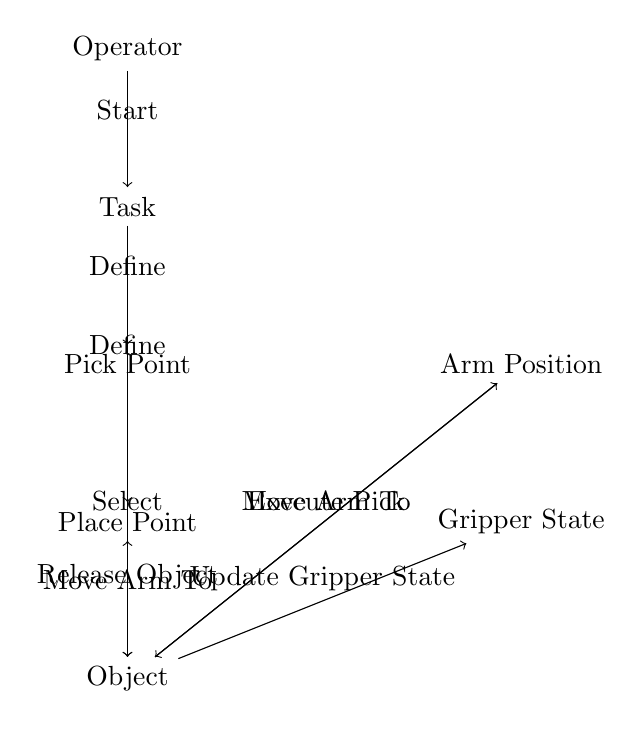
\begin{tikzpicture}[node distance=2cm, auto]

    % Nodes
    \node (Operator) {Operator};
    \node (Task) [below of=Operator] {Task};
    \node (PickPoint) [below of=Task] {Pick Point};
    \node (PlacePoint) [below of=PickPoint] {Place Point};
    \node (Object) [below of=PlacePoint] {Object};
    \node (ArmPosition) [right of=PickPoint, xshift=3cm] {Arm Position};
    \node (GripperState) [right of=PlacePoint, xshift=3cm] {Gripper State};

    % Edges
    \draw[->] (Operator) -- node[above] {Start} (Task);
    \draw[->] (Task) -- node[above] {Define} (PickPoint);
    \draw[->] (Task) -- node[above] {Define} (PlacePoint);
    \draw[->] (PickPoint) -- node[above] {Select} (Object);
    \draw[->] (Object) -- node[above] {Move Arm To} (ArmPosition);
    \draw[->] (ArmPosition) -- node[above] {Execute Pick} (Object);
    \draw[->] (Object) -- node[above] {Move Arm To} (PlacePoint);
    \draw[->] (PlacePoint) -- node[above] {Release Object} (Object);
    \draw[->] (Object) -- node[above] {Update Gripper State} (GripperState);

\end{tikzpicture}

\end{document}